\section{Datenbankschema}
\label{sec:db}
Zu Beginn der Entwicklung kam \textit{SQLite} als Datenbankmanagementsystem zum Einsatz. Es stellte sich jedoch heraus, dass es zu Problemen bei gleichzeitigem Zugriff auf die Datenbank kommt. Daher kommt momentan \textit{MySQL} zum Einsatz. MySQL ist weit verbreitetes Datenbankmanagementsystem, ist es Open Source und frei verfügbar. Mit mehreren Datenbankverbindungen kommt es problemlos aus. Das System wird auf dem gleichen Host wie der Webserver für die Datenrepräsentation und der Webservice für die Datenbereitstellung ausgeführt. Dieser externe Server läuft in einer virtuellen Maschine der DHBW Karlsruhe. Das Betriebssystem des Server ist ein Ubuntu-Server. 
\begin{figure}[h!]
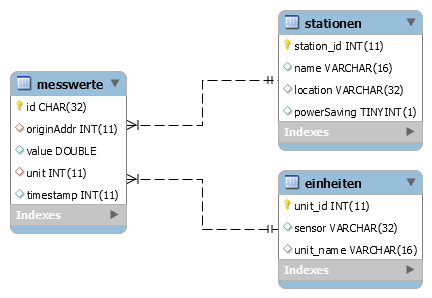
\includegraphics[scale=0.8]{bilder/EERDiagramm} 
\caption{Schema der Datenbank}
\label{Datenbankschema}
\end{figure}   
Die Datenbank beinhaltet drei Tabellen. Bei dem Attribut \textit{id} vom Typ CHAR(32) in der Tablle \textit{messwerte} handelt es sich um die gehashte ID. Diese Tabelle enthält die eigentlichen Messdaten. Die ID dient als Primarykey. Das Attribut \textit{originAddr} gibt an von welchem Sensorknoten (Arduino) das Tupel stammt. \textit{value} gibt den Messwert der entsprechenden Messgröße beziehungsweise Einheit (\textit{unit}) an. Der \textit{timestamp} ist im UNIX-Format. Er zählt die Sekunden seit dem ersten 01.01.1970 hoch. Diese Datumsrepräsentation ist besonders simpel. Da die Arduinos keine Echtzeituhr haben, erstellt der Raspberry Pi beim Empfang den Zeitstempel.
Die Attribute \textit{originAddr} und \textit{unit} sind in \textit{messwerte} sind jeweils Fremdschlüssel. \textit{originAddr} ist Primärschlüssel in der Tabelle \textit{stationen}. Sie dient der Speicherung aller Sensorknoten. Die Tabelle enthält außerdem noch die Spalte \textit{name}, den Standort (\textit{location}) und ein Flag (\textit{powerSavig}), ob es sich um einen energiesparenden Arduino handelt oder nicht.
\textit{einheiten} hat als eindeutigen Primärschlüssel \textit{unit\_id}. In der Tabelle sind alle Messgrößen enthalten. Ein String (VARCHAR(32)) bezeichnet den Sensor (zum Beispiel Luftfeuchte). \textit{unit\_name} repräsentiert die Einheit der Messgröße (zum Beispiel \textit{\%}) 
